\onecolumn

\appendix




\section{Proofs for Section \ref{sec:alg}} \label{apx:proof}
\begin{proof}[Proof of Prop. \ref{prop:uprime-size}]
  Let $m^* = \left( 1 + \frac{\kappa }{\delta c_{min} } \right) \log ( n / \epsi ) + 1.$
  
  First, we show that at any time during the execution of Alg. \ref{alg:single}, $|A| \le m^* + |A_s|$.
  Fix a value $B$ of $A_s$, and let $A_i, 1 \le i \le m$ assume all distinct values of $A$ while $A_s$
  has value $B$, in the order in which they were assigned. Thus, $A_1 = A_s$, $A_2 = A_s + e_1, \ldots, A_m = A_s + e_1 + \ldots + e_{m-1}$.
  Then, let $(y_i = f(A_i))_{i=1}^m$. By Line \ref{line:add}, $y_i \ge \left( 1 + \frac{\delta c_{min}}{\kappa } \right) y_{i-1}$, for each $i \in [m]$. Let $\beta = \frac{\delta c_{min}}{\kappa }$; then by Fact \ref{fact:1}, if $i \ge m^* - 1$, then $y_i \ge \frac{n}{\epsi} y_1$, and a deletion is triggered on Line \ref{line:delete}, which changes the value of $A_s$. Hence, we have $m \le m^*$, which shows $|A| \le |A_s| = m^*$.

  Observe that after a deletion, $|A_s| = m \le m^*$. Since $A_s$ has initial value $\emptyset$, it holds that $|A_s| \le m^*$ throughout the execution of the algorithm. Therefore, $|A| \le 2m^*$, and thus $|\uni'| \le 2m^* +1$. 
\end{proof}
\begin{proof}[Proof of Prop. \ref{prop:ahat-adot}]
  Let $( \dot B_i )_{i=1}^m$ be the sequence of sets deleted by the algorithm on
  Line \ref{line:delete-set}, in the order in which they were deleted.
  Let $j(i)$ be the iteration of the \textbf{for} loop on which $B_i$
  was deleted, and let $A_{j(i)}$ be the value of the set $A$ at the
  beginning of iteration $j(i)$. Let $B_0 = \hat A$, and let
  $B_i = B_{i-1} \setminus \hat B_i$, for $i = 1$ to $m$.
  Observe that $B_m = \dot A$.

  We have that
  \begin{align*}
    f( B_{i-1} ) - f(B_i) &\overset{(a)}{\le} \gamma^{-1} f( \dot B_i ) \\
                          &\overset{(b)}{<} \frac{\gamma^{-1}\epsi}{n} f( A_{j(i)} ) \\
                          &\overset{(c)}{\le} \frac{\gamma^{-1}\epsi}{n} f( \hat A ),
  \end{align*}
  where Inequality (a) follows from $\gamma$-submodularity,
  Inequality (b) is from the condition to delete set $\dot B_i$ on Line \ref{line:delete},
  and Inequality (c) follows from monotonicity.
  From here,
  \begin{align*}
    f( \hat A ) - f( \dot A ) &= \sum_{i=1}^m f( B_{i-1} ) - f( B_i ) \\
    &\le m \cdot \frac{\gamma^{-1}\epsi}{n} f( \hat A ) \le \gamma^{-1}\epsi f( \hat A ). \qedhere
  \end{align*}
\end{proof}
\begin{proof}[Proof of Lemma \ref{lemma:value-inside-A}]
  If $c(A_m) \le \kappa$, let $A^* = A_m$ and there is nothing to show.
  Otherwise, let $A' =  \{a_{i'}, \ldots, a_m \}$, where $i' = \max_{i \in [m]} \{ i: c( \{ a_i, \ldots, a_m \} ) > \kappa \}$.
  We have
  \begin{align*}
    f(A') &\overset{(a)}{\ge} \gamma ( f(A_m) - f( A_m \setminus A') ) \\
          &\overset{(b)}{=} \gamma \sum_{i=i'}^m \marge{ a_i }{ A_{i-1} } \\
          &\overset{(c)}{\ge} \gamma^2 \sum_{i=i'}^m \frac{ \delta c(a_i) f( A_{i-1} )}{\kappa} \\
          &\overset{(d)}{>} \gamma^2 \delta f(A_{i'-1} ) = \gamma^2 \delta f( A \setminus A' ),
  \end{align*}
  where Inequality (a) follows from $\gamma$-submodularity and nonnegativity, Equality (b)
  is a telescoping sum, Inequality (c) is from the assumed condition (2), and Inequality
  (d) is from monotonicity and the fact that $c( A' ) > \kappa$.
  Thus
  \begin{align*}
    f(A_m) &\le \gamma^{-1} (f(A') + f( A_m \setminus A')) \\
           &< \gamma^{-1}(1 + 1/(\delta \gamma^2 )) f(A') = \frac{\delta \gamma^2  +1}{\delta \gamma^3 } f(A').
  \end{align*}
  Let $A'' = A' \setminus a_{i'}$; by choice of $A'$, it holds that $c(A'') \le \kappa$.
  Finally, from $\gamma$-submodularity,
  \begin{align*}
    f(a^*) + f(A'') &\ge f(a_{i'}) + f(A'') \\
                    &\ge \gamma f(A') \ge \frac{\delta \gamma^4}{\delta \gamma^2 + 1} f(A_m).
  \end{align*}
  % $$f( a^* ) + f(A'') \ge f(a_{i'}) + f(A'') \ge \gamma f(A') \ge \frac{\delta \gamma^4}{\delta \gamma^2 + 1} f(A_m).$$ 
  Thus, set $A^* = \argmax \{ f( a^* ), f(A'') \}$. 
\end{proof}
\begin{proof}[Proof of Prof. \ref{prop:aprime}]
  Let $\dot A = \{\dot a_1, \ldots, \dot a_m \}$ be in the order in which the elements were added into set $A$.
  That is, if $j(i)$ the iteration of the \textbf{for} loop in which $\dot a_i$ is considered, $i < i'$ implies
  $j(i) < j(i')$. Let $A_j$ be the value of the set $A$ at the beginning of iteration $j$ of the \textbf{for}
  loop.
  Then
  \begin{align*}
    \marge{ \dot a_i }{ \dot A_{i-1} } &\overset{(a)}{\ge} \gamma \marge{ \dot a_i }{ A_{j(i)} } \\
                                       &\overset{(b)}{\ge} \gamma \frac{ \delta c( \dot a_i ) f( A_{j(i)} )}{\kappa} \\
                                       &\overset{(c)}{\ge} \gamma \frac{ \delta c( \dot a_i ) f( \dot A_{i - 1} )}{\kappa},
  \end{align*}
  where (a) follows from $\gamma$-submodularity since $\dot A_{i-1} \subseteq A_{j(i)}$,
  (b) follows from the condition on Line \ref{line:add},
  (c) follows from monotonicity. 
  Also $c(\dot a_i ) \le \kappa$, for all $i$. Therefore, $\dot A_i$ and $a^*$ satisfy the conditions of
  Lemma \ref{lemma:value-inside-A}, which implies the result. 
\end{proof}
\begin{proof}[Proof of Prop. \ref{prop:opt-ahat}]
  Let $O \subseteq \uni$, such that $c(O) \le \kappa$ and $f(O) = \opt$.
  For each $e \in \uni$, let $j(e)$ be the iteration of the \textbf{for}
  loop in which $e$ was considered, and let $A_j$ be the value of the set
  $A$ at the beginning of the $j$th iteration. 
  Then
  \begin{align*}
    \opt - f( \hat A ) &\overset{(a)}{\le } f( O \cup \hat A ) - f( \hat A) \\
                       &\overset{(b)}{\le } \gamma^{-1} \sum_{o \in O \setminus \hat A} \marge{o}{ A_{j(o)} } \\
                       &\overset{(c)}{<} \gamma^{-1} \sum_{o \in O \setminus \hat A} \frac{\delta c(o) f(A_{j(o)})}{\kappa } \\
                       &\overset{(d)}{\le} \gamma^{-1} \sum_{o \in O \setminus \hat A} \frac{\delta c(o) f( \hat A )}{\kappa } \\
                       &\overset{(e)}{\le} \gamma^{-1} \delta f( \hat A ),
  \end{align*}
  where (a) follows from monotonicity,
  (b) follows from $\gamma$-submodularity,
  (c) holds since the condition on Line \ref{line:add} must have failed since $o \not \in \hat A$,
  (d) follows from monotonicity, and (e) holds since $\sum_{o \in O} c(o) \le \kappa$.
\end{proof}
\begin{proof}[Proof of Prop. \ref{prop:part}] 
  Let $X \subseteq O$ be a maximal subset with $c(X) \le \kappa ( 1 - \eta )$.
  By Assumption \nhi, $X \neq \emptyset$. If $X = O$, there is nothing to show.
  Otherwise, let $o \in O \setminus X$. By definition, $c \left( O \setminus (X \cup \{ o \} \right) < \kappa - \kappa ( 1 - \eta ) = \eta \kappa < (1 - \eta) \kappa$, since $\eta \le 1/2$. Therefore, $O_1 = X$, $O_2 = \{ o \}$, and $O_3 = O \setminus (X \cup \{ o \} )$
  form the requisite partition. 
\end{proof}
\section{Experimental Setup} We run all our experiments on a Linux server equipped with an NVIDIA RTX A6000 GPU and an AMD EPYC $7713$ CPU, using PyTorch $2.4.1$ and Python $3.12.7$. Code and data are available at: \url{https://github.com/ankurnath/QuickPrune}.

\section{Problem Formulation}\label{appendix:problem_formulation}
In this section, we formally introduce the four applications mentioned in the paper. A CO problem on graph can be described with an undirected graph $G (V, E)$, where $V$ is the set of vertices, $E$ is the set of edges and each node $v \in V$ is associated with a cost $c(v)$. For knapsack constraint, we set the cost of each node $v \in V$ as $c(v) = \frac{\beta}{|V|} (|N(v)| - \alpha) $ where $N(v)$ is the set of neighbors of $v$ , $\alpha = \frac{1}{20}$ and $\beta$ is a normalizing factor so $c(v) \geq 1$,  so that the cost of each node is roughly proportional to the value of the node following \citet{yaroslavtsev2020bring}.

\textbf{Maximum Cover.} Given a budget $k$ , the goal of this problem is to find a subset of nodes $S \subseteq V$ that maximizes the objective function, $f(S)= |\{v |  v \in S \lor \exists(u,v) \in E , u \in S  \}|$ where $ \sum_{v \in S} c(v) \leq k$.

\textbf{Maximum Cut (MaxCut).} Given a budget $k$, the goal of this problem is to find a subset of nodes $S \subseteq V$ that maximizes the objective function, $f(S)= |\{ (u,v) \in E: v \in S, u \in V \setminus S \}|$ where $ \sum_{v \in S} c(v) \leq k$.

\textbf{Influence Maximization (IM).} Given a budget $k$, probabilities $p(u,v)$ on the edges $(u,v)\in E$ and a cascade model $\mathcal{C}$, the goal of this problem is to find a subset of nodes $S \subseteq V$ that maximizes the expected spread, $f(S)= \mathbf{E}[\sigma(S)]$ where $\sigma(S)$ denotes the spread of $S$ and $ \sum_{v \in S} c(v) \leq k$.  For the experiments, we consider the independent cascade model \citep{kempe2003maximizing} and set $p = 0.01$ following \citet{chen2009efficient}. Because relatively large propagation probability $p$ the influence spread is not very sensitive to different algorithms and heuristics, because a giant connected component exists even after removing every edge with probability $1-p$.

\textbf{Information Retrieval System.} Given a budget $k$, a set of candidate items $C$ (images or videos), and a set of query items $Q$, the objective is to find a subset $S \in C$ that maximizes the graph cut function, $f(S) = \lambda \sum_{i \in Q} \sum_{j \in S} s(i,j) - \sum_{i,j \in S} s(i,j) $  where $s$ is the similarity kernel and $\lambda \geq 2$. We set $\lambda = 10$ for our experiments. Note that the condition on $\lambda$ is to ensure that $f$ remains a monotone submodular function \cite{iyer2021submodular}. For video recommendation, the constraint is $\sum_{v \in S} L(v) \leq k$, where $L(v)$ represents the length of a video normalized the minimum length of the video. For the image retrieval system, the constraint is simply $|S| \leq k$.


\section{Baselines} \label{appendix:baselines}
In this section, we provide details about each algorithm discussed in our paper.



\textbf{GCOMB-P.} The idea is as follows: For a graph $G_{i} = (V, E)$ from training distribution and a budget of $b$, the vertices are initially sorted into descending order based on the sum of outgoing edge-weight (or degree in an unweighted graph), and $rank(v)$ denotes the position of vertex $v$ in this ordered list. A stochastic solver is used $m$ times to obtain $m$ different solution sets $ \{S^{(1)},S^{(2)},...,S^{(m)}\} $ for budget $b$. The goal here is to predict all nodes that could potentially be part of the solution set.  We define $r^{G_i}_{b}= \max_{v \in \cup_{j} S^{(j)}} rank(v)$ to be the highest rank of all vertices among the vertices in each of the $m$ solution sets. We repeat this process for each graph in the training distribution and define $r_{b} = \max_{G_i \in G_{train}} r^{G_i}_{b}$ for budget $b$. To generalize across budgets, we compute $r_b$ for a series of budgets and obtain $(b,r_b)$ pairs. To generalize across graph sizes, budgets and ranks are normalized with respect to the number of nodes in the graph. During testing, for an unseen budget $b$, linear interpolation is used to predict $r_b$.

% For Max Cover, \citet{manchanda2020gcomb} proposed a novel probabilistic greedy algorithm, and for IM, \citet{manchanda2020gcomb} used IMM \cite{tang2015influence} as the stochastic solvers. 


\textbf{LeNSE.} \citet{ireland2022lense} proposed extracting a small portion of the original graph that most likely contains the optimal solution, where the solution can be extracted using any existing heuristics. The idea is as follows: Given a training distribution, extract the optimal solutions for each graph. Next, generate random subgraphs containing different portions of nodes from the optimal solution, where subgraphs are sets of nodes and their 1-hop neighbors. Assign these subgraphs to different classes based on the ratio of the objective function value from the subgraph to that of the original graph. The number of classes depends on the problem and dataset and usually requires domain knowledge.
In the next step, a reinforcement learning agent is trained to navigate a subgraph induced by a fixed number of random nodes and their 1-hop neighbors, updating the subgraph at each step by replacing a single vertex with its neighbors. By updating the subgraph in this manner, the agent aims to obtain a subgraph close to the optimal subgraph in the embedding space created by the encoder.

\textbf{Submodular Sparsification (SS).}   \citet{zhou2017scaling} proposed a randomized pruning method to reduce the submodular maximization problem via a novel concept called the submodularity graph. The submodularity graph is a weighted directed graph \( G(V,E,w) \) defined by a normalized submodular function \( f: 2^{V} \rightarrow \mathcal{R_+} \), where \( V \) is the set of nodes corresponding to the ground set, and each directed edge \( (u,v) \in E \) has weight \( w(u,v) = f(v \mid u) - f(u \mid V \setminus u) \). As computing all edge weights is quadratic in complexity, they proposed a randomized approach. The idea is as follows: Sample a subset of random nodes from the original ground set, remove these random nodes from the ground set at each step, and add them to the pruned ground set. Then, remove a subset of the top elements from the ground set that are deemed unimportant from the sample nodes in that set. After several stages of pruning, when the original ground set size falls below a certain threshold, the remaining elements are merged with the pruned ground set.

\textbf{COMBHelper.}  \citet{tian2024combhelper} introduced a method to train a GNN for vertex classification in combinatorial problems, predicting nodes likely to be part of the solution. To improve scalability, they applied knowledge distillation to transfer knowledge to a smaller GNN and used problem specific weight boosting to enhance the performance. 


% \citet{tian2024combhelper} introduced a method that trains a GNN to predict nodes likely to be part of the solution in combinatorial problems. Their approach focuses on vertex classification, under the assumption that nodes in the solution exhibit similar properties. To enhance scalability, they used knowledge distillation to transfer knowledge to a smaller GNN, making it more efficient. Additionally, they applied weight boosting techniques to further improve the performance of the model.



\textbf{GNNPruner.} We propose a modified version of \comb, in which we similarly train a vertex GNN classifier to predict solution nodes. Like \comb and \lense, we generate training labels using solutions from  a heuristic. However, unlike these methods, we use random numbers as node features for experiments under size constraints, and replace SAGEConv \citep{hamilton2017inductive} with a lightweight GCN \citep{kipf2016semi} with fewer layers. Empirical evidence shows that this architectural shift helps capture structural relationships in the graph without relying on the handcrafted features used by \comb and \lense. Additionally, it improves scalability by using fewer layers. We simplify prepossessing and improve prediction accuracy through more generalized learning by leveraging random features (shown in Table \ref{tab:size_constraint}). However, in experiments involving knapsack constraints, instead of using random numbers as node features, we provide the degree, cost, and the degree-to-cost ratio of each node as input features. This adjustment appears to improve performance.
\section{Dataset Information} \label{appendix:dataset}

In Table \ref{tab:dataset_distribution}, we list the graphs used in our empirical evaluations along with the sizes of the respective training and testing splits for the traditional CO problems on graphs. We follow \citet{ireland2022lense} to determine what percentage of the original graph edges was used for training and testing.

\begin{table}[h]
\centering
\caption{The real-world graphs used to perform our experiments. 
% For each graph, we provide the corresponding size of the training and
% testing sets; in brackets we indicate the percentage of edges taken from the original graph for training purposes with the remaining edges
% being used to form the test graph.
}

\vspace{1em}
\begin{tabular}{|c|c|c|c|c|}
\hline
         & \multicolumn{2}{c|}{Train Size}        & \multicolumn{2}{c|}{Test Size}           \\ \cline{2-5} 
Graph    & \multicolumn{1}{c|}{Vertices} & Edges  & \multicolumn{1}{c|}{Vertices} & Edges    \\ \hline
Facebook & 3847                          & $26470 (30\%)$  & 4002                          & 61764    \\
Wiki     & 4891                          & $30228 (30\%)$  & 6358                          & 70534    \\
Deezer   & 48870                         & $149460 (30\%)$& 53511                         & 348742   \\
SlashDot & 47546                         & $140566 (30\%)$& 67640                         & 327988   \\
Twitter  & 55827                         & $134229 (10\%)$& 80712                         & 1208067  \\
DBLP     & 63004                         & $41994 (10\%)$ & 315305                        & 1007872  \\
YouTube  & 185193                        & $179257 (06\%)$ & 1098104                       & 2808367  \\
Skitter  & 147604                        & $110952 (01\%)$ & 1694318                       & 10984346 \\ \hline
\end{tabular}

\label{tab:dataset_distribution}
\end{table}


For the information retrieval problem, we use the Beans dataset \citep{beansdata}, CIFAR100 \citep{Krizhevsky09learningmultiple}, FOOD101 \citep{bossard14}, and UCF101 \citep{soomro2012ucf101dataset101human}. Since the Beans dataset contains only three classes, we undersample one class to make the problem more challenging and use that class for querying. For the FOOD101 dataset, we sample 100 images per food category for our candidate set and query from the test dataset. Similarly, for the UCF-101 dataset, we select 100 videos for each action and randomly query from the validation dataset.






\section{Network architectures and hyper-parameters}



\paragraph{QuickPrune.} For all graph problem experiments, we set $\delta = 0.1$, $\epsilon = 0.1$, and $\eta = 0.5$. In the knapsack-constrained MaxCover experiment, we set $\delta = 0.5$. For both image and video retrieval systems, we use $\delta = 0.05$, $\epsilon = 0.1$, and $\eta = 0.5$.


\paragraph{SS.} For all experiments, we set $r=8$ and $c=8$, following \citet{zhou2017scaling}. We find that this configuration empirically performs well.


\paragraph{GNNPruner.} The architecture consists of two layers, each containing a graph convolutional layer with ReLU activation and $16 $ hidden channels. We use the Adam optimizer with a learning rate of $0.001$ and a weight decay of $5 \times 10^{-4}$, training with cross-entropy loss. At each epoch, we randomly sample vertices both from the solution and non-solution sets to prevent the loss from being dominated by the non-solution vertices. 





\section{Efficiency and scalability analysis} \label{appendix:scalability}

From Figure \ref{fig:memory_comparsion} , we observe that most algorithms (\qs, SS, \gcomb) only utilize CPU resources. Algorithms like \lense, \comb, and \gnn use both CPU and GPU resources, with \comb showing the highest combined usage, making it the most computationally demanding algorithm , followed by GNNPruner; in contrast, LeNSE exhibits relatively minimal usage. LeNSE only modifies a subgraph, so it does not need to load the entire graph into the memory.

\begin{figure}
    \centering
    
\includegraphics[width=0.5\linewidth]{Figures/cpu_gpu_usage_by_algorithm_inkspace.pdf}
    \caption{Average GPU and CPU memory utilization among
algorithms for MaxCover on YouTube dataset.}
    \label{fig:memory_comparsion}
\end{figure}

We also report the runtime for MaxCover on each dataset in Table \ref{tab:runtime}. For other constraints and applications, the results are qualitatively similar.
% Please add the following required packages to your document preamble:
% \usepackage{booktabs}
\begin{table}[]
\centering
\caption{Comparison of the runtime (in seconds) of algorithms across different datasets for MaxCover.}
\vspace{1em}
\label{tab:runtime}
\begin{tabular}{@{}|c|c|c|c|c|c|c|c|c|@{}}
% \toprule
\hline
Algorithm         & Facebook & Wiki   & Deezer & Slashdot & Twitter & DBLP    & YouTube & Skitter  \\ \hline
\textbf{QuickPrune (OURS)} & 0.064    & 0.094  & 0.437  & 0.590    & 1.075   & 1.208   & 5.443   & 10.317   \\
SS                & 3.178    & 5.804  & 41.995 & 58.281   & 120.555 & 168.011 & 769.871 & 2238.035 \\
GNNpruner         & 1.073    & 1.272  & 6.741  & 6.654    & 17.222  & 15.157  & 48.702  & 162.288  \\
CombHelper        & 1.071    & 1.195  & 5.997  & 5.964    & 15.914  & 14.644  & 47.352  & NA       \\
GCOMB-P           & 0.002    & 0.004  & 0.026  & 0.039    & 0.058   & 0.197   & 0.501   & 0.982    \\
LeNSE             & 27.024   & 25.238 & 34.210 & 38.315   & 76.827  & 38.325  & 231.557 & 1593.406 \\ 
% \bottomrule
\hline
\end{tabular}
\end{table}


\section{Additional table and plots}




In this section, you can find the tables and plots omitted in the main paper due to space constraints.
\subsection{Heuristics}\label{appendix:heuristics}

In Table \ref{tab:dataset_distribution}, we summarize the algorithms used for each application under size and knapsack constraints. Note that for the knapsack-constrained experiments for IM, we use the improved greedy heuristic (referred to as Algorithm 2 in the original paper) from \citet{nguyen2013budgeted}.
\begin{table}[h]
\centering
\caption{Summary of Heuristic Approaches}
\vspace{1em}
\label{tab:heuristics}

\begin{tabular}{lll}
\toprule
Problem   & Size            & Knapsack                 \\ \midrule
MaxCover  & \citet{DBLP:journals/mp/NemhauserWF78}                & \citet{khuller1999budgeted} \\
MaxCut    & \citet{DBLP:journals/mp/NemhauserWF78}                 &   \citet{pham2023linear}   \\
IM        & \citet{tang2015influence} & \citet{nguyen2013budgeted} \\
Retrieval & \citet{DBLP:journals/mp/NemhauserWF78}                & \citet{khuller1999budgeted}                 \\ \bottomrule
\end{tabular}%

\end{table}


\newpage


\subsection{Image and Video Retrieval System.} \label{appendix:retrieval}

In Figure \ref{fig:retrival_system}, we present the results for information retrieval system. We employ the cosine similarity metric to assess the similarity between two images. Instead of using a generalist model trained on large datasets, we use a model fine-tuned on the specific dataset. This approach allows the underlying model to better understand the input images.

\begin{figure*}[h] \label{fig:retrival_system} %{l}{0.6\textwidth}

  \subfigure []{ %\label{fig:depend}
    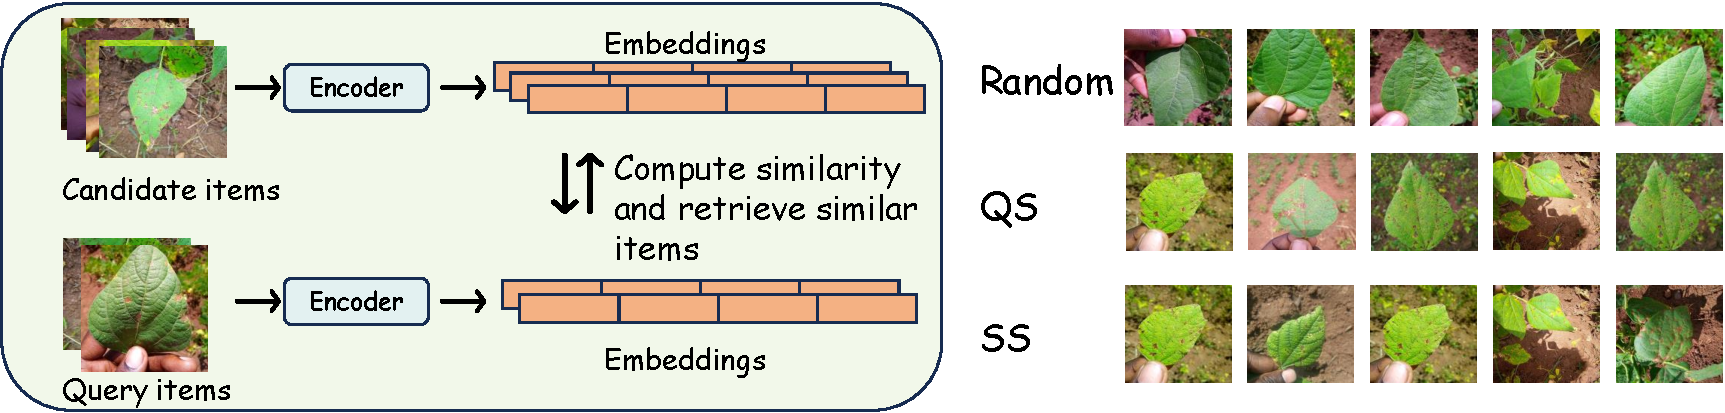
\includegraphics[width=\textwidth]{Figures/retrieval system/retrieval_system_crop_inkspace.pdf}
  }
  \subfigure []{ %\label{fig:depend}
    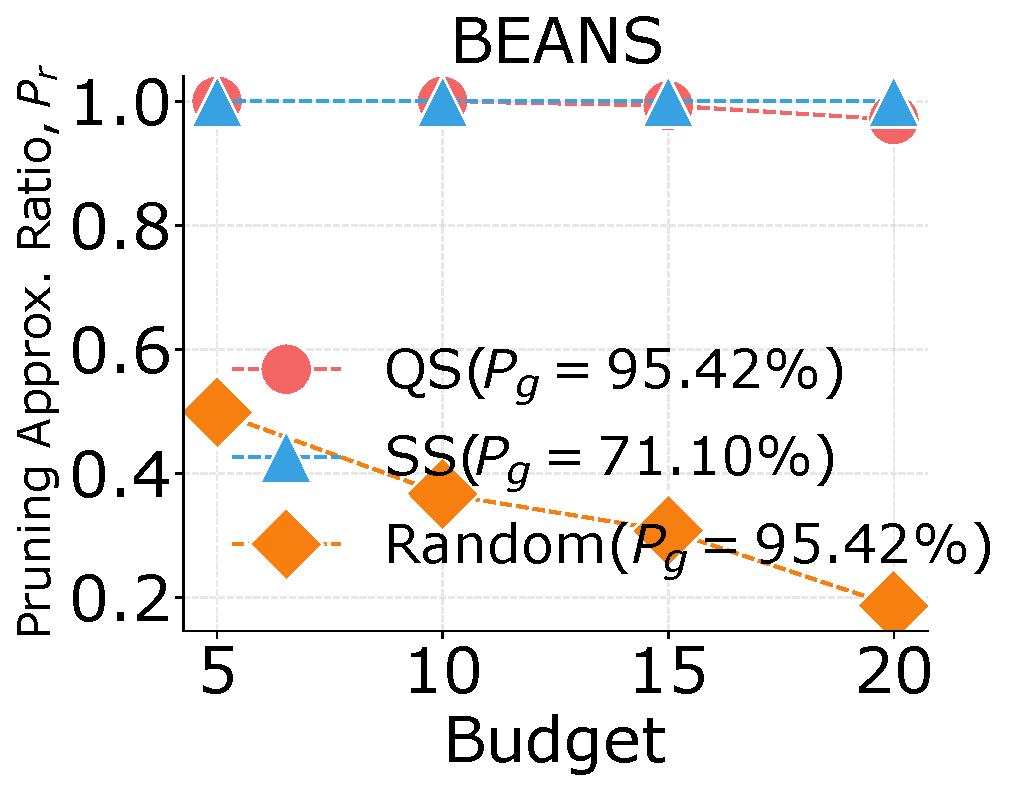
\includegraphics[width=0.23\textwidth]{Figures/retrieval system/BEANS_inkspace.pdf}
  }
  \subfigure[]{ %\label{fig:depend}
    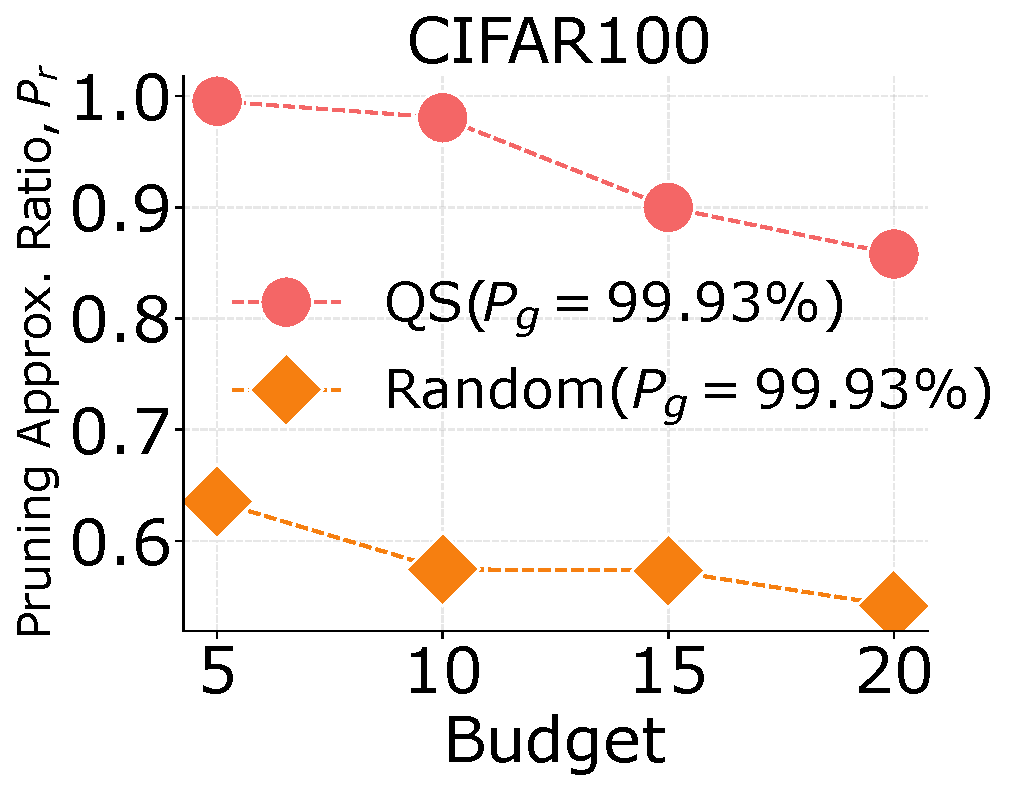
\includegraphics[width=0.23\textwidth]{Figures/retrieval system/CIFAR100_inkspace.pdf}
  }
  \subfigure[]{ %\label{fig:depend}
    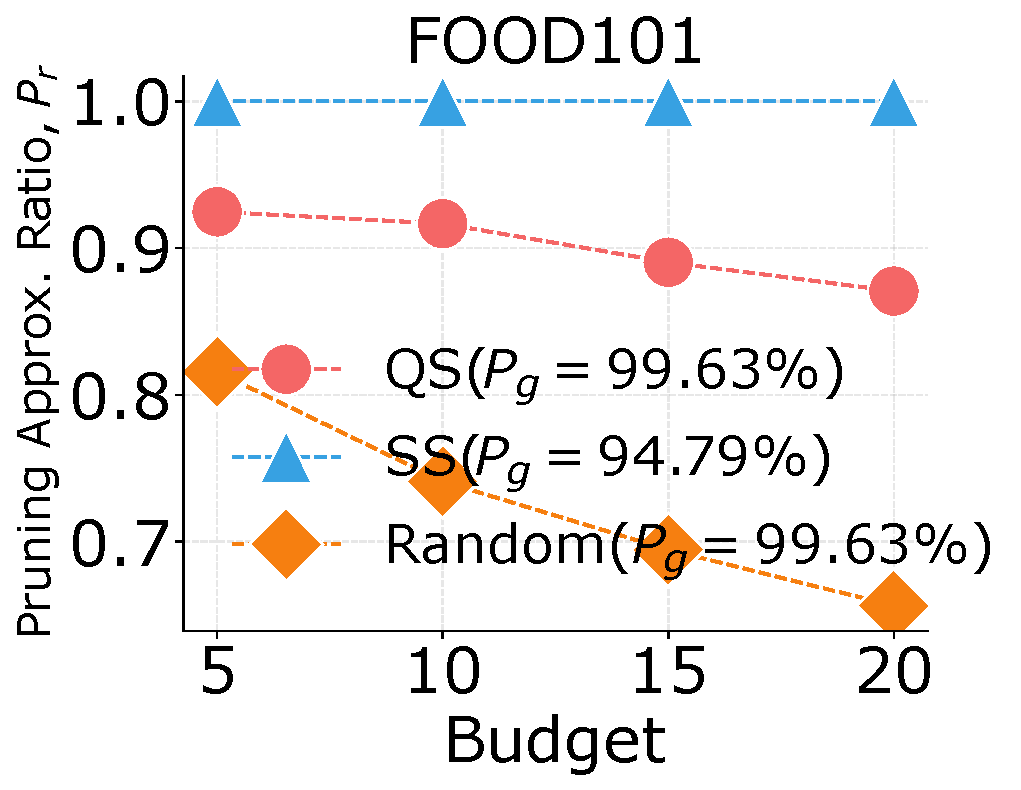
\includegraphics[width=0.23\textwidth]{Figures/retrieval system/FOOD101_inkspace.pdf}
  }
    \subfigure[]{ \label{fig:video_summ}
    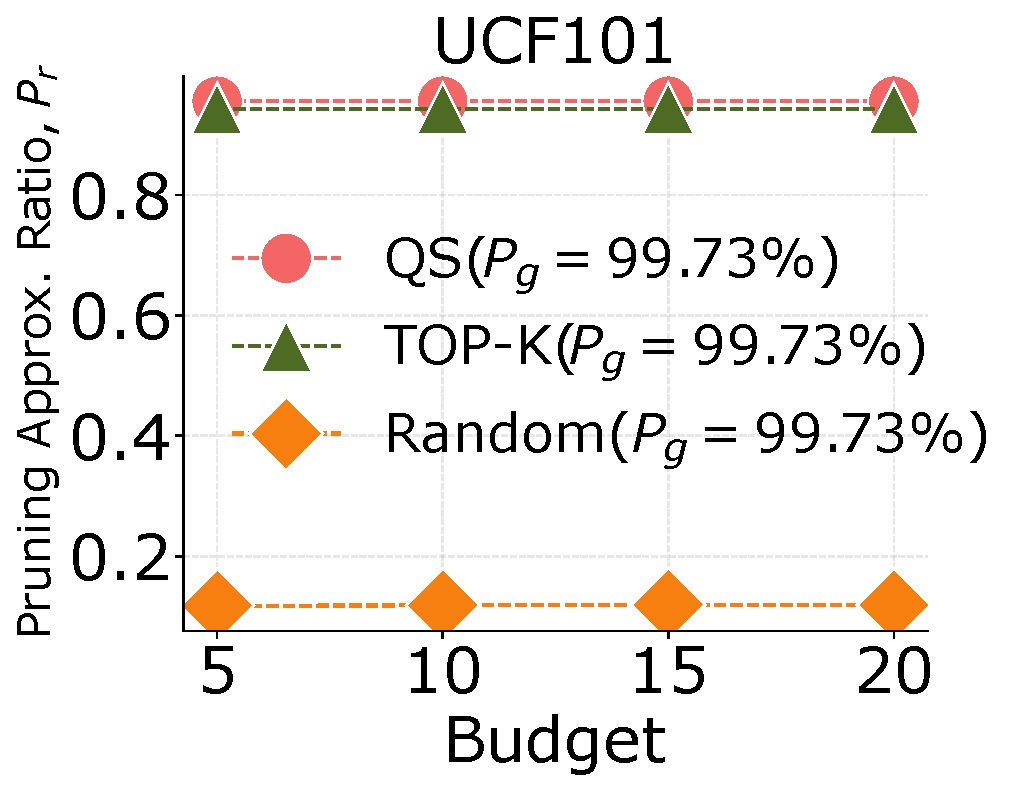
\includegraphics[width=0.23\textwidth]{Figures/retrieval system/UCF101_inkspace.pdf}
  }


  
  \caption{Retrieval system: (a) The pipeline of the retrieval system and a visual representation of images selected by various algorithms for the Beans Dataset. (b-e) Multi-budget analysis of the retrieval system for budgets ranging from $5$ to $20$. Note that $P_g$ represents the percentage of the ground set that has been pruned.}
  

\end{figure*}

\subsection{Knapsack constrained experiments} \label{appendix:qs_vs_baselines_IM}

In Table \ref{tab:knapsack_constraint},  we present the results of our experiments under knapsack constraint.

\begin{table}[h]
\centering
\caption{Comparison of pruning algorithms for knapsack constraint experiments (best combined metric in bold).}
\label{tab:knapsack_constraint}
\vspace{1em}
\begin{tabular}{|cccccccccc|}
\hline
\multicolumn{1}{|c|}{}         & \multicolumn{3}{c|}{\qs}                                              & \multicolumn{3}{c|}{\topk}                                           & \multicolumn{3}{c|}{\gnn}                       \\ \hline
\multicolumn{1}{|c|}{Graph}    & $P_r \uparrow$ & $P_g$ $\uparrow$ & \multicolumn{1}{c|}{$C \uparrow$} & $P_r \uparrow$ & $P_g$ $\uparrow$ & \multicolumn{1}{c|}{$C\uparrow$} & $P_r \uparrow$ & $P_g$ $\uparrow$ & $C\uparrow$ \\ \hline
& \multicolumn{9}{c|}{\textbf{Maximum Cover}}  \\ \hline
 \multicolumn{1}{|c|}{Facebook} 
& 0.9725& 0.9871& \multicolumn{1}{c|}
{\textbf{0.9600}}& 0.5505& 0.9871& \multicolumn{1}{c|}
{0.5434}& 0.3303& 0.9936& \multicolumn{1}{c|}
{0.3282} \\
 \multicolumn{1}{|c|}{Wiki} 
& 0.9400& 0.9851& \multicolumn{1}{c|}
{\textbf{0.9260}}& 0.7550& 0.9851& \multicolumn{1}{c|}
{0.7438}& 1.0000& 0.8696& \multicolumn{1}{c|}
{0.8696} \\
 \multicolumn{1}{|c|}{Deezer} 
& 0.8750& 0.9983& \multicolumn{1}{c|}
{0.8735}& 0.9150& 0.9983& \multicolumn{1}{c|}
{0.9134}& 1.0000& 0.9725& \multicolumn{1}{c|}
{\textbf{0.9725}} \\
 \multicolumn{1}{|c|}{Slashdot} 
& 0.8950& 0.9988& \multicolumn{1}{c|}
{\textbf{0.8939}}& 0.5700& 0.9988& \multicolumn{1}{c|}
{0.5693}& 1.0000& 0.8325& \multicolumn{1}{c|}
{0.8325} \\
 \multicolumn{1}{|c|}{Twitter} 
& 0.8700& 0.9987& \multicolumn{1}{c|}
{\textbf{0.8689}}& 0.5950& 0.9987& \multicolumn{1}{c|}
{0.5942}& 1.0000& 0.4783& \multicolumn{1}{c|}
{0.4783} \\
 \multicolumn{1}{|c|}{DBLP} 
& 0.8450& 0.9997& \multicolumn{1}{c|}
{0.8447}& 0.7150& 0.9997& \multicolumn{1}{c|}
{0.7148}& 1.0000& 0.9971& \multicolumn{1}{c|}
{\textbf{0.9971}} \\
 \multicolumn{1}{|c|}{YouTube} 
& 0.9150& 0.9999& \multicolumn{1}{c|}
{\textbf{0.9149}}& 0.5200& 0.9999& \multicolumn{1}{c|}
{0.5199}& 1.0000& 0.3626& \multicolumn{1}{c|}
{0.3626} \\
 \multicolumn{1}{|c|}{Skitter} 
& 0.9050& 0.9999& \multicolumn{1}{c|}
{0.9049}& 0.8150& 0.9999& \multicolumn{1}{c|}
{0.8149}& 1.0000& 0.9887& \multicolumn{1}{c|}
{\textbf{0.9887}} \\
\hline
& \multicolumn{9}{c|}{\textbf{Maximum Cut}}  \\ \hline
 \multicolumn{1}{|c|}{Facebook} 
& 0.9899& 0.9666& \multicolumn{1}{c|}
{0.9568}& 1.0000& 0.9666& \multicolumn{1}{c|}
{0.9666}& 0.9697& 0.4984& \multicolumn{1}{c|}
{0.4833} \\
 \multicolumn{1}{|c|}{Wiki} 
& 0.9600& 0.9928& \multicolumn{1}{c|}
{\textbf{0.9531}}& 0.5100& 0.9928& \multicolumn{1}{c|}
{0.5063}& 1.0000& 0.1836& \multicolumn{1}{c|}
{0.1836} \\
 \multicolumn{1}{|c|}{Deezer} 
& 0.9600& 0.9985& \multicolumn{1}{c|}
{0.9586}& 0.8000& 0.9985& \multicolumn{1}{c|}
{0.7988}& 1.0000& 0.9745& \multicolumn{1}{c|}
{\textbf{0.9745}} \\
 \multicolumn{1}{|c|}{Slashdot} 
& 0.9700& 0.9991& \multicolumn{1}{c|}
{\textbf{0.9691}}& 0.6700& 0.9991& \multicolumn{1}{c|}
{0.6694}& 1.0000& 0.4395& \multicolumn{1}{c|}
{0.4395} \\
 \multicolumn{1}{|c|}{Twitter} 
& 0.9500& 0.9996& \multicolumn{1}{c|}
{0.9496}& 0.2900& 0.9996& \multicolumn{1}{c|}
{0.2899}& 1.0000& 0.0222& \multicolumn{1}{c|}
{0.0222} \\
 \multicolumn{1}{|c|}{DBLP} 
& 0.9500& 0.9999& \multicolumn{1}{c|}
{0.9499}& 0.4300& 0.9999& \multicolumn{1}{c|}
{0.4300}& 1.0000& 0.9988& \multicolumn{1}{c|}
{\textbf{0.9988}} \\
 \multicolumn{1}{|c|}{YouTube} 
& 0.9700& 0.9999& \multicolumn{1}{c|}
{\textbf{0.9699}}& 0.7300& 0.9999& \multicolumn{1}{c|}
{0.7299}& 1.0000& 0.9406& \multicolumn{1}{c|}
{0.9406} \\
 \multicolumn{1}{|c|}{Skitter} 
& 0.9700& 0.9999& \multicolumn{1}{c|}
{0.9699}& 1.0000& 0.9999& \multicolumn{1}{c|}
{\textbf{0.9999}}& 1.0000& 0.9993& \multicolumn{1}{c|}
{0.9993} \\
\hline
& \multicolumn{9}{c|}{\textbf{Influence Maximization}}  \\ \hline
 \multicolumn{1}{|c|}{Facebook} 
& 0.9934& 0.9148& \multicolumn{1}{c|}
{\textbf{0.9088}}& 0.9934& 0.9148& \multicolumn{1}{c|}
{\textbf{0.9088}}& 0.1173& 0.9854& \multicolumn{1}{c|}
{0.1156} \\
 \multicolumn{1}{|c|}{Wiki} 
& 0.9660& 0.8774& \multicolumn{1}{c|}
{0.8476}& 1.0000& 0.8774& \multicolumn{1}{c|}
{\textbf{0.8774}}& 0.8280& 0.8491& \multicolumn{1}{c|}
{0.7031} \\
 \multicolumn{1}{|c|}{Deezer} 
& 1.0000& 0.9820& \multicolumn{1}{c|}
{\textbf{0.9820}}& 1.0000& 0.9820& \multicolumn{1}{c|}
{\textbf{0.9820}}& 0.4678& 0.9719& \multicolumn{1}{c|}
{0.4547} \\
 \multicolumn{1}{|c|}{Slashdot} 
& 0.9132& 0.9868& \multicolumn{1}{c|}
{0.9011}& 1.0120& 0.9868& \multicolumn{1}{c|}
{\textbf{0.9986}}& 0.7385& 0.8403& \multicolumn{1}{c|}
{0.6206} \\
 \multicolumn{1}{|c|}{Twitter} 
& 0.9121& 0.9986& \multicolumn{1}{c|}
{0.9108}& 0.9689& 0.9986& \multicolumn{1}{c|}
{\textbf{0.9675}}&  0.1399 & 0.9999 & \multicolumn{1}{c|}
{0.1398} \\
 \multicolumn{1}{|c|}{DBLP} 
& 1.0000& 0.9958& \multicolumn{1}{c|}
{0.9958}& 1.0000& 0.9958& \multicolumn{1}{c|}
{0.9958}& 1.0000& 0.9999& \multicolumn{1}{c|}
{\textbf{0.9999}} \\
 \multicolumn{1}{|c|}{YouTube} 
& 0.9171& 0.9994& \multicolumn{1}{c|}
{0.9165}& 0.9502& 0.9994& \multicolumn{1}{c|}
{\textbf{0.9496}}& 0.9814& 0.3299& \multicolumn{1}{c|}
{0.3238} \\
\multicolumn{1}{|c|}{Skitter}  &    0.8291            &     0.9999             &           \multicolumn{1}{c|}
{0.8290}                        &   0.9391             &    0.9999               &    \multicolumn{1}{c|}
{\textbf{0.9390}}                              &    0.9999            &    0.1399              &     0.1398        \\ \hline
\end{tabular}%

\end{table}



\subsection{Comparison between \qs and \qss} \label{appendix:multi_vs_single}

In this section, we present the comparison between \qs and \qss under knapsack constraint. We run \qss with the maximum budget in the range (in our case, this would be 100).

\begin{figure*}[] %{l}{0.6\textwidth}
  \subfigure { %\label{fig:depend}
    
\includegraphics[width=0.23\textwidth]{Figures/MaxCover/Facebook_inkspace.pdf}
  }
  \subfigure{ %\label{fig:depend}
    
\includegraphics[width=0.23\textwidth]{Figures/MaxCover/Wiki_inkspace.pdf}
  }
  \subfigure{ %\label{fig:depend}
    
\includegraphics[width=0.23\textwidth]{Figures/MaxCover/Deezer_inkspace.pdf}
  }
    \subfigure{ %\label{fig:depend}
    
\includegraphics[width=0.23\textwidth]{Figures/MaxCover/Slashdot_inkspace.pdf}
  }
  \subfigure { %\label{fig:depend}
    
\includegraphics[width=0.23\textwidth]{Figures/MaxCover/Twitter_inkspace.pdf}
  }
  \subfigure{ %\label{fig:depend}
    
\includegraphics[width=0.23\textwidth]{Figures/MaxCover/DBLP_inkspace.pdf}
  }
  \subfigure{ %\label{fig:depend}
    
\includegraphics[width=0.23\textwidth]{Figures/MaxCover/YouTube_inkspace.pdf}
  }
    \subfigure{ %\label{fig:depend}
    
\includegraphics[width=0.23\textwidth]{Figures/MaxCover/Skitter_inkspace.pdf}
  }

  
  \caption{Multi-Budget vs Single Budget for MaxCover}
  \label{}

\end{figure*}

\begin{figure*}[t] %{l}{0.6\textwidth}
  \subfigure { %\label{fig:depend}
    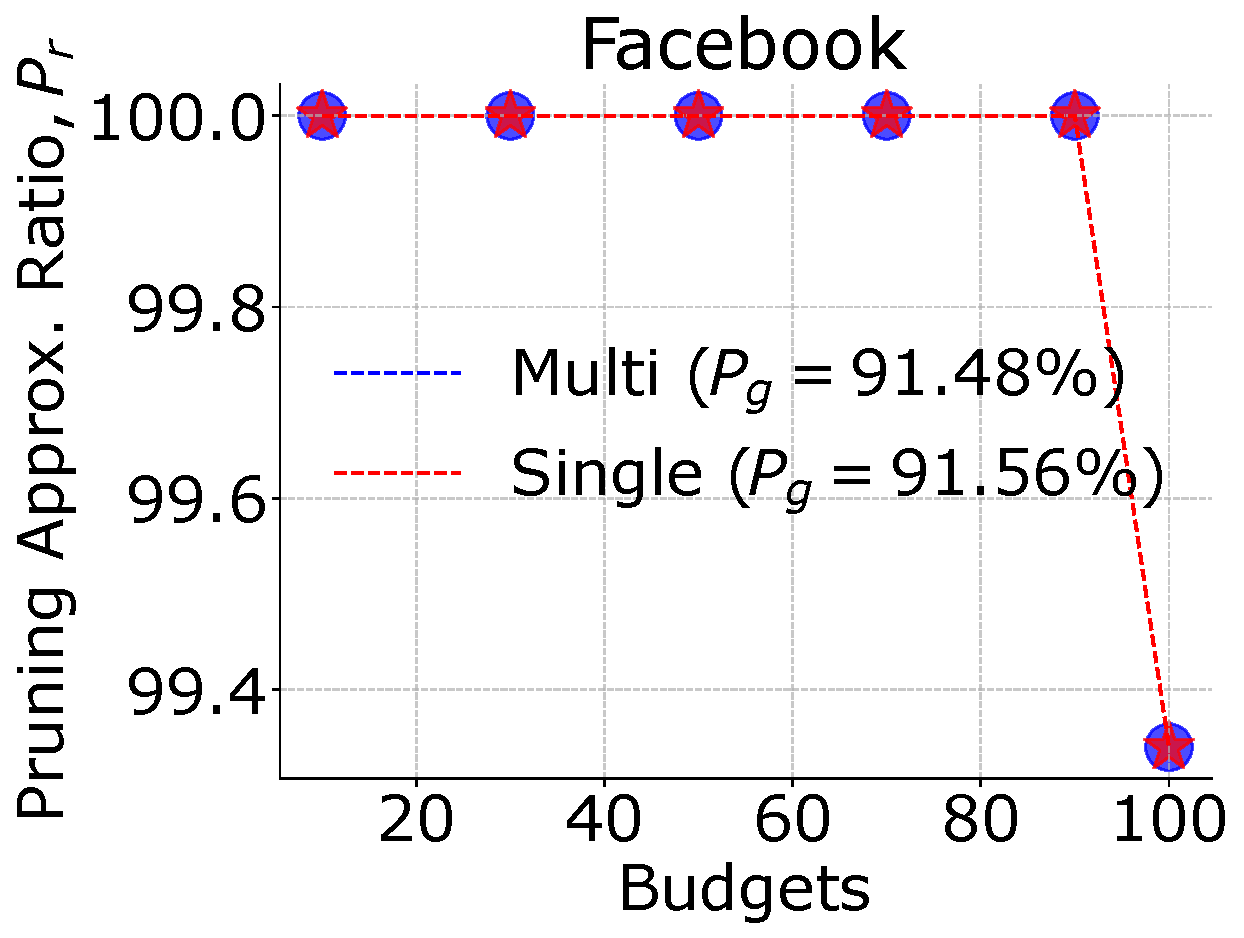
\includegraphics[width=0.23\textwidth]{Figures/IM/Facebook_inkspace.pdf}
  }
  \subfigure{ %\label{fig:depend}
    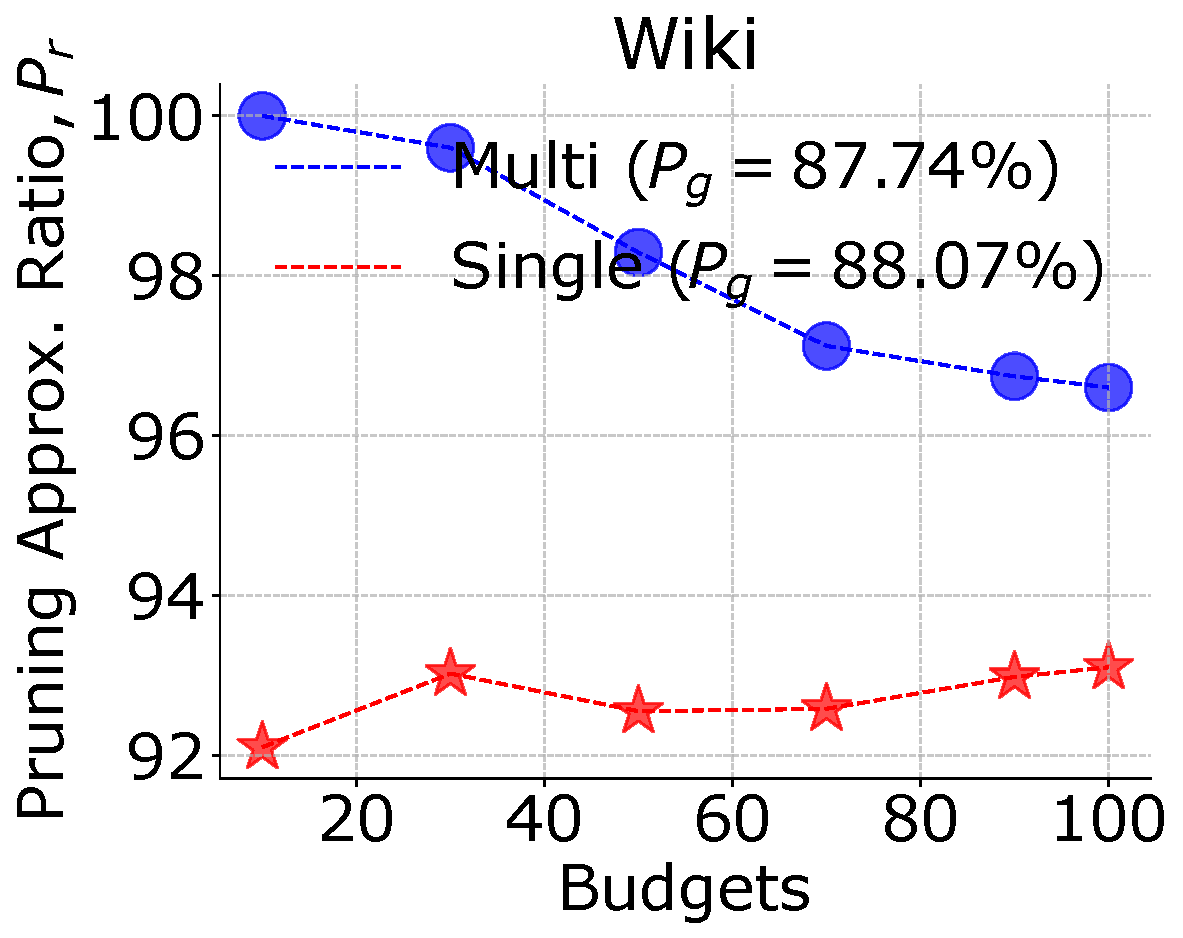
\includegraphics[width=0.23\textwidth]{Figures/IM/Wiki_inkspace.pdf}
  }
  \subfigure{ %\label{fig:depend}
    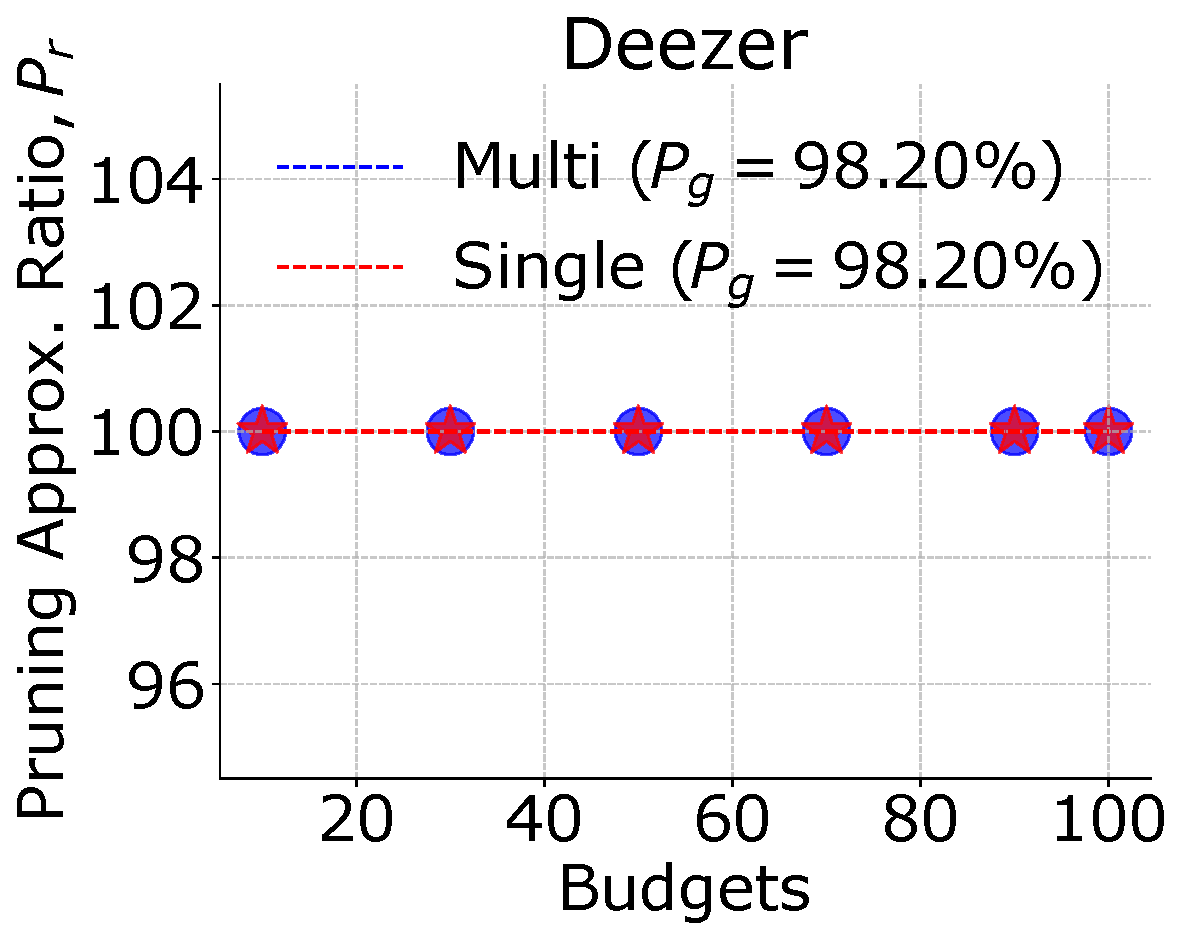
\includegraphics[width=0.23\textwidth]{Figures/IM/Deezer_inkspace.pdf}
  }
    \subfigure{ %\label{fig:depend}
    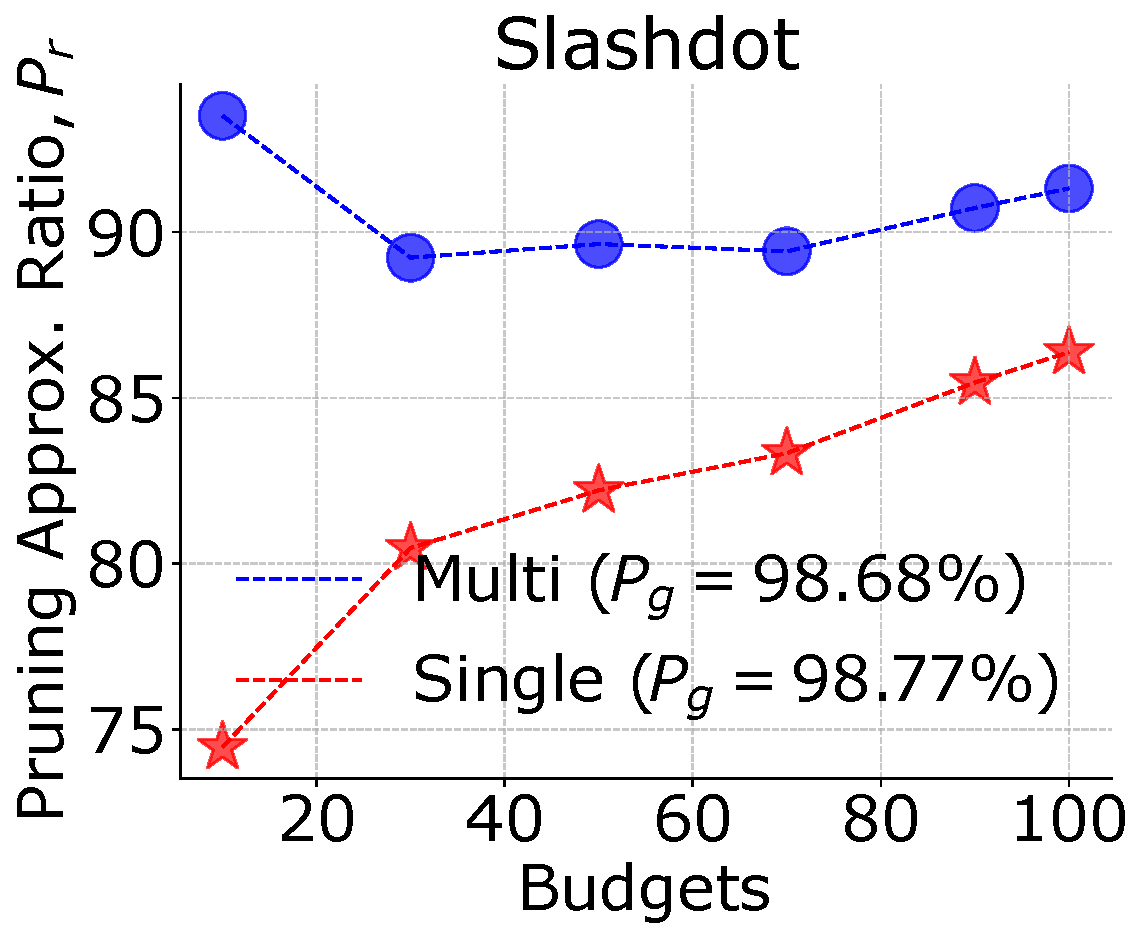
\includegraphics[width=0.23\textwidth]{Figures/IM/Slashdot_inkspace.pdf}
  }
  \subfigure { %\label{fig:depend}
    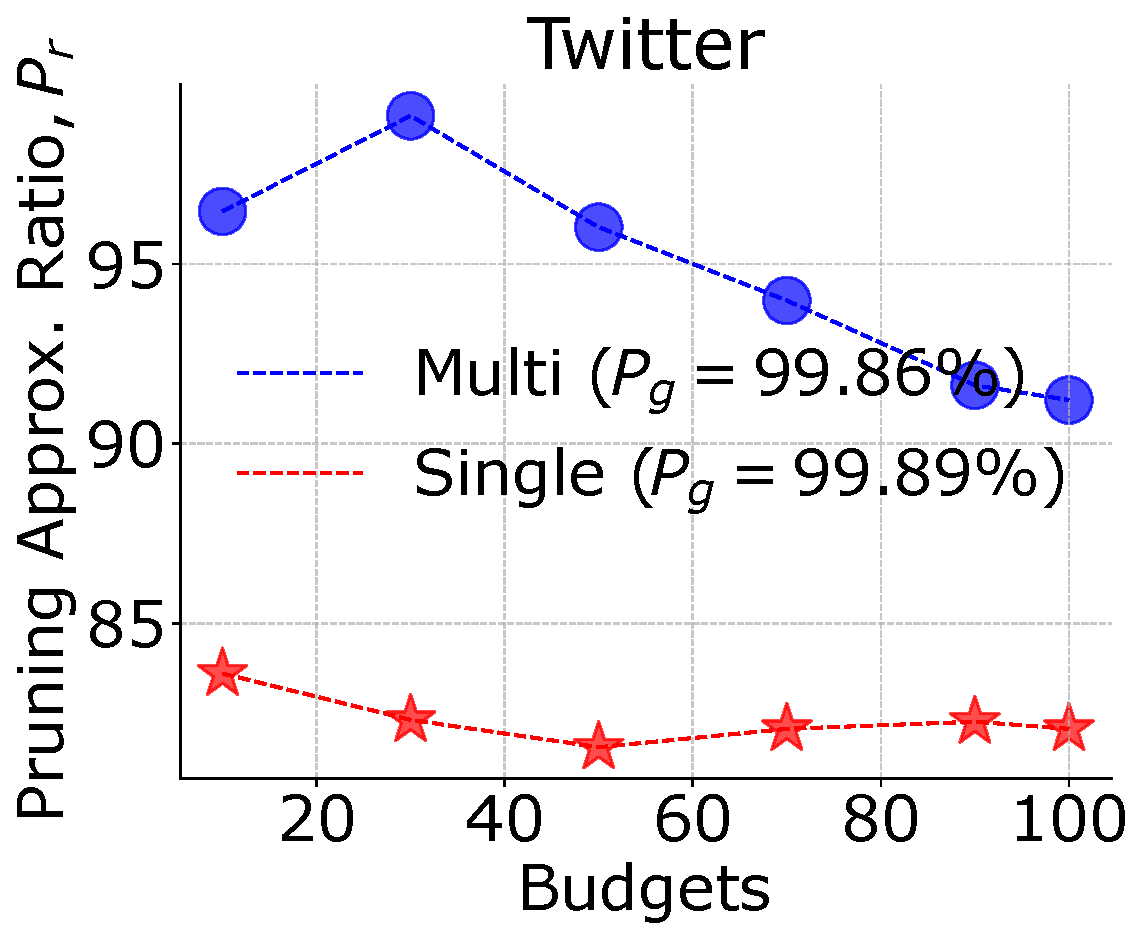
\includegraphics[width=0.23\textwidth]{Figures/IM/Twitter_inkspace.pdf}
  }
  \subfigure{ %\label{fig:depend}
    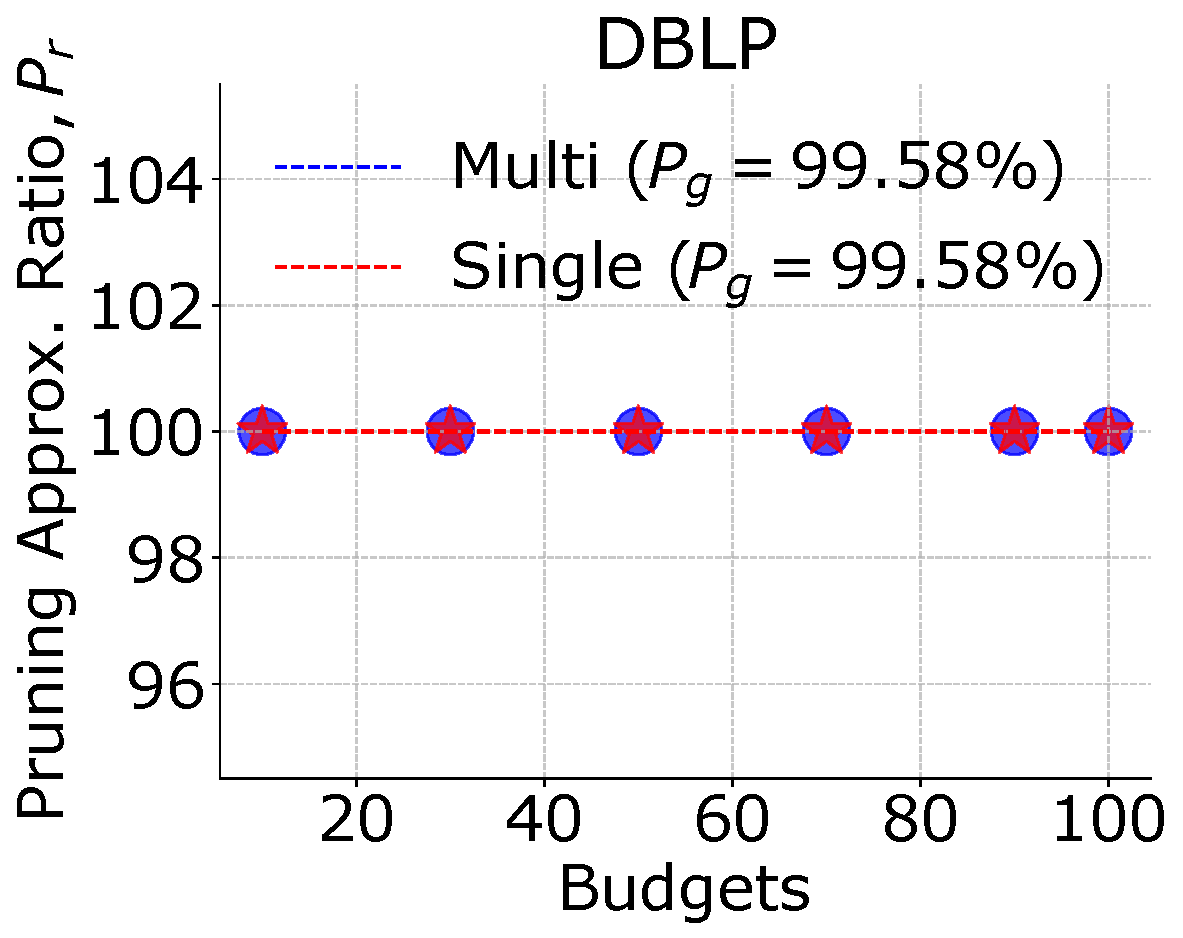
\includegraphics[width=0.23\textwidth]{Figures/IM/DBLP_inkspace.pdf}
  }
  \subfigure{ %\label{fig:depend}
    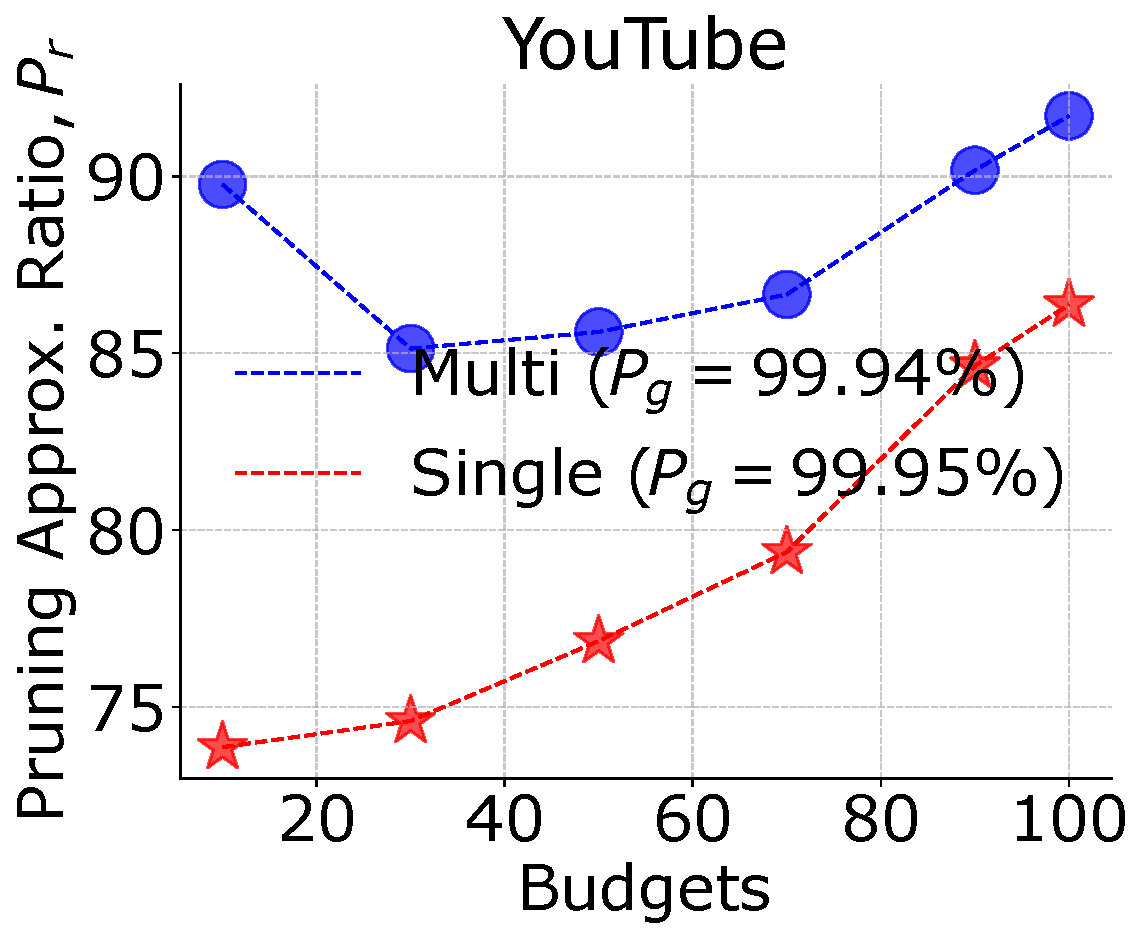
\includegraphics[width=0.23\textwidth]{Figures/IM/YouTube_inkspace.pdf}
  }
  \subfigure{ %\label{fig:depend}
    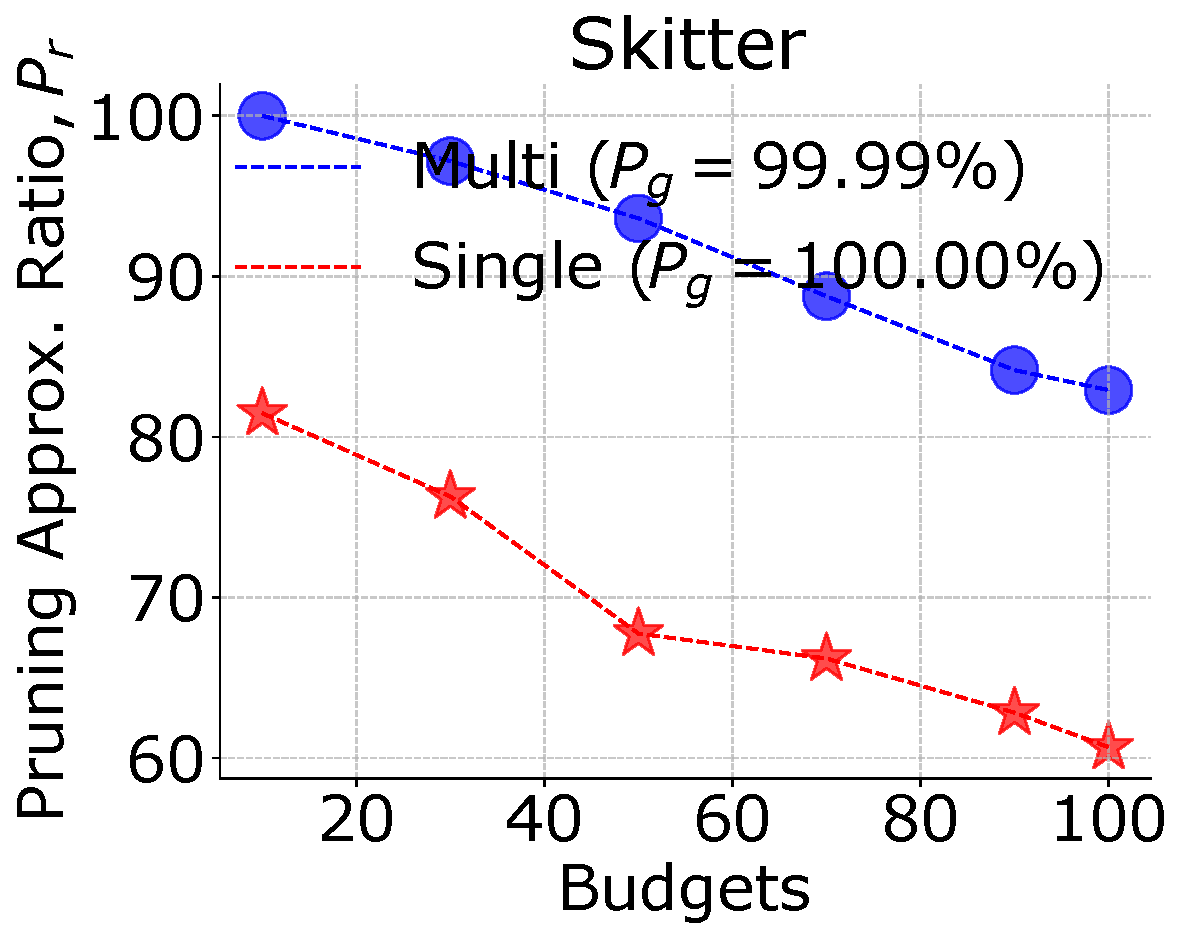
\includegraphics[width=0.23\textwidth]{Figures/IM/Skitter_inkspace.pdf}
  }

  
  \caption{Multi-Budget vs Single Budget for IM}
  \label{}

\end{figure*}


\begin{figure*}[t] %{l}{0.6\textwidth}
  \subfigure { %\label{fig:depend}
    
\includegraphics[width=0.23\textwidth]{Figures/MaxCut/Facebook_inkspace.pdf}
  }
  \subfigure{ %\label{fig:depend}
    
\includegraphics[width=0.23\textwidth]{Figures/MaxCut/Wiki_inkspace.pdf}
  }
  \subfigure{ %\label{fig:depend}
    
\includegraphics[width=0.23\textwidth]{Figures/MaxCut/Deezer_inkspace.pdf}
  }
    \subfigure{ %\label{fig:depend}
    
\includegraphics[width=0.23\textwidth]{Figures/MaxCut/Slashdot_inkspace.pdf}
  }
  \subfigure { %\label{fig:depend}
    
\includegraphics[width=0.23\textwidth]{Figures/MaxCut/Twitter_inkspace.pdf}
  }
  \subfigure{ %\label{fig:depend}
    
\includegraphics[width=0.23\textwidth]{Figures/MaxCut/DBLP_inkspace.pdf}
  }
  \subfigure{ %\label{fig:depend}
    
\includegraphics[width=0.23\textwidth]{Figures/MaxCut/YouTube_inkspace.pdf}
  }
    \subfigure{ %\label{fig:depend}
    
\includegraphics[width=0.23\textwidth]{Figures/MaxCut/Skitter_inkspace.pdf}
  }
  % \subfigure[WS] { %\label{fig:depend}
  %   \includegraphics[width=0.31\textwidth]{Experiments/Maximum_Cut/ObjectiveMCWatts_Strogatz.pdf}
  % }
  % \subfigure[WS] { %\label{fig:depend}
  %   \includegraphics[width=0.31\textwidth]{Experiments/Maximum_Cut/QueriesMCWatts_Strogatz.pdf}
  % }
  
  \caption{Multi-Budget vs Single Budget for MaxCut}
  \label{}

\end{figure*}




% Please add the following required packages to your document preamble:
% \usepackage{graphicx}
% Please add the following required packages to your document preamble:
% \usepackage{graphicx}
% \begin{table*}[h]
% \centering
% \caption{Comparison of pruning algorithms for size constraint experiments (best in bold); *Values as reported in  \cite{ireland2022lense} and ``--" denotes no reasonable result is achieved by the corresponding algorithm under the time constraint.\todo{add combined metric and move some algs. to appendix.}}
% \vspace{1em}
% \label{tab:size_constraint}
% \resizebox{\textwidth}{!}{%
% \begin{tabular}{|ccccccccccccc|}
% \hline
% \multicolumn{1}{|c||}{}         & \multicolumn{2}{c||}{\qs}                                & \multicolumn{2}{c||}{SS}                                 & \multicolumn{2}{c||}{\gcomb*}                           & \multicolumn{2}{c||}{\comb}                              & \multicolumn{2}{c||}{\lense*}                           & \multicolumn{2}{c|}{\gnn}          \\ \hline
% \multicolumn{1}{|c||}{Graph}    & $P_r \uparrow$  & \multicolumn{1}{c||}{$P_g$ $\uparrow$} & $P_r \uparrow$  & \multicolumn{1}{c||}{$P_g$ $\uparrow$} & $P_r \uparrow$ & \multicolumn{1}{c||}{$P_g$ $\uparrow$} & $P_r \uparrow$  & \multicolumn{1}{c||}{$P_g$ $\uparrow$} & $P_r \uparrow$ & \multicolumn{1}{c||}{$P_g$ $\uparrow$} & $P_r \uparrow$  & $P_g$ $\uparrow$ \\ \hline
% \multicolumn{13}{|c|}{\textbf{Max Coverage}}                                                                                                                                                                                                                                                                                                                                 \\ \hline
% \multicolumn{1}{|c||}{Facebook} & \textbf{100.0}  & \multicolumn{1}{c||}{\textbf{99.53}}   & \textbf{100.0}  & \multicolumn{1}{c||}{90.27}            & 92.7           & \multicolumn{1}{c||}{7.00}             & \textbf{100.0}  & \multicolumn{1}{c||}{38.40}            & 96.6           & \multicolumn{1}{c||}{7.00}             & \textbf{100.0}  & 76.97            \\
% \multicolumn{1}{|c||}{Wiki}     & 99.98           & \multicolumn{1}{c||}{\textbf{94.22}}   & 95.35           & \multicolumn{1}{c||}{93.46}            & 99.0           & \multicolumn{1}{c||}{3.00}             & 100.0           & \multicolumn{1}{c||}{45.28}            & \textbf{109.4} & \multicolumn{1}{c||}{34.00}            & 100.0           & 91.99            \\
% \multicolumn{1}{|c||}{Deezer}   & 96.06           & \multicolumn{1}{c||}{97.97}            & 98.55           & \multicolumn{1}{c||}{\textbf{98.55}}   & 99.4           & \multicolumn{1}{c||}{13.00}            & \textbf{100.0}  & \multicolumn{1}{c||}{72.78}            & 97.9           & \multicolumn{1}{c||}{75.00}            & \textbf{100.0}  & 91.51            \\
% \multicolumn{1}{|c||}{Slashdot} & \textbf{100.0}  & \multicolumn{1}{c||}{\textbf{99.25}}   & 98.02           & \multicolumn{1}{c||}{98.89}            & \textbf{100.0} & \multicolumn{1}{c||}{2.00}             & \textbf{100.0}  & \multicolumn{1}{c||}{98.44}            & 97.9           & \multicolumn{1}{c||}{69.00}            & \textbf{100.0}  & 98.20            \\
% \multicolumn{1}{|c||}{Twitter}  & 99.29           & \multicolumn{1}{c||}{\textbf{99.11}}   & 93.50           & \multicolumn{1}{c||}{98.93}            & 99.7           & \multicolumn{1}{c||}{17.00}            & \textbf{100.0}  & \multicolumn{1}{c||}{56.54}            & 98.9           & \multicolumn{1}{c||}{33.00}            & 99.87           & 97.93            \\
% \multicolumn{1}{|c||}{DBLP}     & 99.51          & \multicolumn{1}{c||}{99.57}            & 99.64           & \multicolumn{1}{c||}{\textbf{99.63}}   & 99.9           & \multicolumn{1}{c||}{3.00}             & \textbf{100.0}  & \multicolumn{1}{c||}{18.18}            & 99.0           & \multicolumn{1}{c||}{90.00}            & \textbf{100.0}  & 87.05            \\
% \multicolumn{1}{|c||}{YouTube}  & \textbf{100.0}  & \multicolumn{1}{c||}{\textbf{99.95}}   & 99.68           & \multicolumn{1}{c||}{99.87}            & 99.8           & \multicolumn{1}{c||}{7.00}             & 100.00          & \multicolumn{1}{c||}{95.72}            & 98.2           & \multicolumn{1}{c||}{79.00}            & 99.55           & 99.70            \\
% \multicolumn{1}{|c||}{Skitter}  & 99.85           & \multicolumn{1}{c||}{\textbf{99.97}}   & 99.11           & \multicolumn{1}{c||}{99.91}            & \textbf{99.9}  & \multicolumn{1}{c||}{10.00}            & -               & \multicolumn{1}{c||}{-}                & 97.6           & \multicolumn{1}{c||}{70.00}            & 99.93           & 98.91            \\ \hline
% \multicolumn{13}{|c|}{\textbf{Maximum Cut}}                                                                                                                                                                                                                                                                                                                                  \\ \hline
% \multicolumn{1}{|c||}{Facebook} & 98.86           & \multicolumn{1}{c||}{79.35}            & 98.84           & \multicolumn{1}{c||}{90.27}            & 81.30          & \multicolumn{1}{c||}{\textbf{95.00}}   & \textbf{100.0}  & \multicolumn{1}{c||}{15.38}            & 96.00          & \multicolumn{1}{c||}{7.00}             & \textbf{100.0}  & 67.74            \\
% \multicolumn{1}{|c||}{Wiki}     & 99.85           & \multicolumn{1}{c||}{90.37}            & 99.99           & \multicolumn{1}{c||}{93.46}            & 92.00          & \multicolumn{1}{c||}{\textbf{96.00}}   & \textbf{100.0}  & \multicolumn{1}{c||}{93.46}            & 98.10          & \multicolumn{1}{c||}{39.00}            & \textbf{100.0}  & 90.04            \\
% \multicolumn{1}{|c||}{Deezer}   & 99.96           & \multicolumn{1}{c||}{97.30}            & \textbf{100.0}  & \multicolumn{1}{c||}{98.55}            & 85.00          & \multicolumn{1}{c||}{\textbf{99.00}}   & 100             & \multicolumn{1}{c||}{37.54}            & 97.50          & \multicolumn{1}{c||}{74.00}            & \textbf{100.0}  & 91.88            \\
% \multicolumn{1}{|c||}{Slashdot} & \textbf{100.0}  & \multicolumn{1}{c||}{99.04}            & \textbf{100.0}  & \multicolumn{1}{c||}{98.89}            & 63.20          & \multicolumn{1}{c||}{99.00}            & 79.35           & \multicolumn{1}{c||}{\textbf{99.29}}   & 99.00          & \multicolumn{1}{c||}{62.00}            & \textbf{100.0}  & 97.97            \\
% \multicolumn{1}{|c||}{Twitter}  & \textbf{100.0}  & \multicolumn{1}{c||}{\textbf{99.00}}   & \textbf{100.0}  & \multicolumn{1}{c||}{98.93}            & 62.80          & \multicolumn{1}{c||}{\textbf{99.00}}   & \textbf{100.0}  & \multicolumn{1}{c||}{55.42}            & 98.70          & \multicolumn{1}{c||}{48.00}            & \textbf{100.0}  & 97.40            \\
% \multicolumn{1}{|c||}{DBLP}     & \textbf{100.0}  & \multicolumn{1}{c||}{99.54}            & \textbf{100.0}  & \multicolumn{1}{c||}{\textbf{99.63}}   & 64.60          & \multicolumn{1}{c||}{99.00}            & \textbf{100.0}  & \multicolumn{1}{c||}{18.25}            & 99.30          & \multicolumn{1}{c||}{92.00}            & \textbf{100.0}  & 86.23            \\
% \multicolumn{1}{|c||}{YouTube}  & \textbf{100.0}  & \multicolumn{1}{c||}{\textbf{99.94}}   & 99.99           & \multicolumn{1}{c||}{99.87}            & 53.60          & \multicolumn{1}{c||}{99.00}            & 99.90           & \multicolumn{1}{c||}{97.05}            & 98.70          & \multicolumn{1}{c||}{79.00}            & 99.36           & 99.68            \\
% \multicolumn{1}{|c||}{Skitter}  & \textbf{100.0}  & \multicolumn{1}{c||}{\textbf{99.95}}   & \textbf{100.0}  & \multicolumn{1}{c||}{99.91}            & 42.70          & \multicolumn{1}{c||}{99.00}            & -               & \multicolumn{1}{c||}{-}                & 97.4           & \multicolumn{1}{c||}{71.00}            & \textbf{100.0}  & 98.84            \\ \hline
% \multicolumn{13}{|c|}{\textbf{Influence Maximization}}                                                                                                                                                                                                                                                                                                                       \\ \hline
% \multicolumn{1}{|c||}{Facebook} & 99.19           & \multicolumn{1}{c||}{74.50}            & 92.08           & \multicolumn{1}{c||}{\textbf{90.27}}   & 95.1           & \multicolumn{1}{c||}{73.00}            & 100.39          & \multicolumn{1}{c||}{38.48}            & 97.9           & \multicolumn{1}{c||}{9.00}             & \textbf{99.38}  & 49.17            \\
% \multicolumn{1}{|c||}{Wiki}     & \textbf{102.69} & \multicolumn{1}{c||}{88.31}            & 98.63           & \multicolumn{1}{c||}{\textbf{93.46}}   & 96.9           & \multicolumn{1}{c||}{90.00}            & 99.69           & \multicolumn{1}{c||}{60.46}            & 96.0           & \multicolumn{1}{c||}{51.00}            & 100.11          & 89.64            \\
% \multicolumn{1}{|c||}{Deezer}   & 93.84           & \multicolumn{1}{c||}{96.98}            & \textbf{102.62} & \multicolumn{1}{c||}{\textbf{98.55}}   & 80.5           & \multicolumn{1}{c||}{55.00}            & 98.37           & \multicolumn{1}{c||}{10.93}            & 97.2           & \multicolumn{1}{c||}{76.00}            & 99.84           & 84.78            \\
% \multicolumn{1}{|c||}{Slashdot} & 99.84           & \multicolumn{1}{c||}{98.81}   & 99.59           & \multicolumn{1}{c||}{\textbf{98.89}}            & 96.6           & \multicolumn{1}{c||}{98.00}            & \textbf{100.76} & \multicolumn{1}{c||}{98.75}            & 96.6           & \multicolumn{1}{c||}{77.00}            & 99.93           & 97.97            \\
% \multicolumn{1}{|c||}{Twitter}  & \textbf{100.45} & \multicolumn{1}{c||}{\textbf{99.65}}   & 95.75           & \multicolumn{1}{c||}{98.89}            & 92.0           & \multicolumn{1}{c||}{98.00}            & 99.72           & \multicolumn{1}{c||}{49.47}            & 96.6           & \multicolumn{1}{c||}{40.00}            & 98.42           & 97.58            \\
% \multicolumn{1}{|c||}{DBLP}     & 86.03           & \multicolumn{1}{c||}{99.46}            & \textbf{104.95} & \multicolumn{1}{c||}{\textbf{99.63}}   & 86.3           & \multicolumn{1}{c||}{99.00}            & 98.73           & \multicolumn{1}{c||}{2.94}             & 96.9           & \multicolumn{1}{c||}{89.00}            & 75.58           & 33.25            \\
% \multicolumn{1}{|c||}{YouTube}  & 96.77           & \multicolumn{1}{c||}{\textbf{99.94}}   & 98.46           & \multicolumn{1}{c||}{99.87}            & 93.3           & \multicolumn{1}{c||}{99.00}            & 99.92           & \multicolumn{1}{c||}{97.05}            & 97.1           & \multicolumn{1}{c||}{75.00}            & \textbf{100.18} & 99.66            \\
% \multicolumn{1}{|c||}{Skitter}  &   98.13              & \multicolumn{1}{c||}{\textbf{99.99}}                 &     100.32            & \multicolumn{1}{c||}{99.91}                 & 88.3           & \multicolumn{1}{c||}{99.00}            & -               & \multicolumn{1}{c||}{-}                & 98.3           & \multicolumn{1}{c||}{78.00}            &  \textbf{100.23}               &         98.89         \\ \hline
% \end{tabular}%
% }
% \end{table*}


% \begin{table*}[h]
% \centering
% \caption{Comparison of pruning algorithms for size constraint experiments (best in bold); *Values as reported in  \cite{ireland2022lense} and ``--" denotes no reasonable result is achieved by the corresponding algorithm under the time constraint.}
% \vspace{1em}
% \label{tab:size_constraint}
% \resizebox{\textwidth}{!}{%
% \begin{tabular}{|ccccccccccccc|}
% \hline
% \multicolumn{1}{|c||}{}         & \multicolumn{2}{c||}{\qs}                                & \multicolumn{2}{c||}{SS}                                 & \multicolumn{2}{c||}{\gcomb*}                           & \multicolumn{2}{c||}{\comb}                              & \multicolumn{2}{c||}{\lense*}                           & \multicolumn{2}{c|}{\gnn}          \\ \hline
% \multicolumn{1}{|c||}{Graph}    & $P_r \uparrow$  & \multicolumn{1}{c||}{$P_g$ $\uparrow$} & $P_r \uparrow$  & \multicolumn{1}{c||}{$P_g$ $\uparrow$} & $P_r \uparrow$ & \multicolumn{1}{c||}{$P_g$ $\uparrow$} & $P_r \uparrow$  & \multicolumn{1}{c||}{$P_g$ $\uparrow$} & $P_r \uparrow$ & \multicolumn{1}{c||}{$P_g$ $\uparrow$} & $P_r \uparrow$  & $P_g$ $\uparrow$ \\ \hline
% \multicolumn{13}{|c|}{\textbf{Max Coverage}}                                                                                                                                                                                                                                                                                                                                 \\ \hline
% \multicolumn{1}{|c||}{Facebook} & \textbf{100.0}  & \multicolumn{1}{c||}{\textbf{99.53}}   & \textbf{100.0}  & \multicolumn{1}{c||}{90.27}            & 92.7           & \multicolumn{1}{c||}{7.00}             & \textbf{100.0}  & \multicolumn{1}{c||}{38.40}            & 96.6           & \multicolumn{1}{c||}{7.00}             & \textbf{100.0}  & 76.97            \\
% \multicolumn{1}{|c||}{Wiki}     & 99.91           & \multicolumn{1}{c||}{\textbf{94.25}}   & 95.35           & \multicolumn{1}{c||}{93.46}            & 99.0           & \multicolumn{1}{c||}{3.00}             & 100.0           & \multicolumn{1}{c||}{45.28}            & \textbf{109.4} & \multicolumn{1}{c||}{34.00}            & 100.0           & 91.99            \\
% \multicolumn{1}{|c||}{Deezer}   & 95.02           & \multicolumn{1}{c||}{98.01}            & 98.55           & \multicolumn{1}{c||}{\textbf{98.55}}   & 99.4           & \multicolumn{1}{c||}{13.00}            & \textbf{100.0}  & \multicolumn{1}{c||}{72.78}            & 97.9           & \multicolumn{1}{c||}{75.00}            & \textbf{100.0}  & 91.51            \\
% \multicolumn{1}{|c||}{Slashdot} & \textbf{100.0}  & \multicolumn{1}{c||}{\textbf{99.25}}   & 98.02           & \multicolumn{1}{c||}{98.89}            & \textbf{100.0} & \multicolumn{1}{c||}{2.00}             & \textbf{100.0}  & \multicolumn{1}{c||}{98.44}            & 97.9           & \multicolumn{1}{c||}{69.00}            & \textbf{100.0}  & 98.20            \\
% \multicolumn{1}{|c||}{Twitter}  & 99.08           & \multicolumn{1}{c||}{\textbf{99.13}}   & 93.50           & \multicolumn{1}{c||}{98.93}            & 99.7           & \multicolumn{1}{c||}{17.00}            & \textbf{100.0}  & \multicolumn{1}{c||}{56.54}            & 98.9           & \multicolumn{1}{c||}{33.00}            & 99.87           & 97.93            \\
% \multicolumn{1}{|c||}{DBLP}     & 99.39           & \multicolumn{1}{c||}{99.57}            & 99.64           & \multicolumn{1}{c||}{\textbf{99.63}}   & 99.9           & \multicolumn{1}{c||}{3.00}             & \textbf{100.0}  & \multicolumn{1}{c||}{18.18}            & 99.0           & \multicolumn{1}{c||}{90.00}            & \textbf{100.0}  & 87.05            \\
% \multicolumn{1}{|c||}{YouTube}  & \textbf{100.0}  & \multicolumn{1}{c||}{\textbf{99.95}}   & 99.68           & \multicolumn{1}{c||}{99.87}            & 99.8           & \multicolumn{1}{c||}{7.00}             & 100.00          & \multicolumn{1}{c||}{95.72}            & 98.2           & \multicolumn{1}{c||}{79.00}            & 99.55           & 99.70            \\
% \multicolumn{1}{|c||}{Skitter}  & 99.85           & \multicolumn{1}{c||}{\textbf{99.97}}   & 99.11           & \multicolumn{1}{c||}{99.91}            & \textbf{99.9}  & \multicolumn{1}{c||}{10.00}            & -               & \multicolumn{1}{c||}{-}                & 97.6           & \multicolumn{1}{c||}{70.00}            & 99.93           & 98.91            \\ \hline
% \multicolumn{13}{|c|}{\textbf{Maximum Cut}}                                                                                                                                                                                                                                                                                                                                  \\ \hline
% \multicolumn{1}{|c||}{Facebook} & 95.96           & \multicolumn{1}{c||}{79.02}            & 98.84           & \multicolumn{1}{c||}{90.27}            & 81.30          & \multicolumn{1}{c||}{\textbf{95.00}}   & \textbf{100.0}  & \multicolumn{1}{c||}{15.38}            & 96.00          & \multicolumn{1}{c||}{7.00}             & \textbf{100.0}  & 67.74            \\
% \multicolumn{1}{|c||}{Wiki}     & 97.13           & \multicolumn{1}{c||}{90.54}            & 99.99           & \multicolumn{1}{c||}{93.46}            & 92.00          & \multicolumn{1}{c||}{\textbf{96.00}}   & \textbf{100.0}  & \multicolumn{1}{c||}{93.46}            & 98.10          & \multicolumn{1}{c||}{39.00}            & \textbf{100.0}  & 90.04            \\
% \multicolumn{1}{|c||}{Deezer}   & 99.96           & \multicolumn{1}{c||}{97.30}            & \textbf{100.0}  & \multicolumn{1}{c||}{98.55}            & 85.00          & \multicolumn{1}{c||}{\textbf{99.00}}   & 100             & \multicolumn{1}{c||}{37.54}            & 97.50          & \multicolumn{1}{c||}{74.00}            & \textbf{100.0}  & 91.88            \\
% \multicolumn{1}{|c||}{Slashdot} & \textbf{100.0}  & \multicolumn{1}{c||}{99.04}            & \textbf{100.0}  & \multicolumn{1}{c||}{98.89}            & 63.20          & \multicolumn{1}{c||}{99.00}            & 79.35           & \multicolumn{1}{c||}{\textbf{99.29}}   & 99.00          & \multicolumn{1}{c||}{62.00}            & \textbf{100.0}  & 97.97            \\
% \multicolumn{1}{|c||}{Twitter}  & \textbf{100.0}  & \multicolumn{1}{c||}{\textbf{99.00}}   & \textbf{100.0}  & \multicolumn{1}{c||}{98.93}            & 62.80          & \multicolumn{1}{c||}{\textbf{99.00}}   & \textbf{100.0}  & \multicolumn{1}{c||}{55.42}            & 98.70          & \multicolumn{1}{c||}{48.00}            & \textbf{100.0}  & 97.40            \\
% \multicolumn{1}{|c||}{DBLP}     & \textbf{100.0}  & \multicolumn{1}{c||}{99.54}            & \textbf{100.0}  & \multicolumn{1}{c||}{\textbf{99.63}}   & 64.60          & \multicolumn{1}{c||}{99.00}            & \textbf{100.0}  & \multicolumn{1}{c||}{18.25}            & 99.30          & \multicolumn{1}{c||}{92.00}            & \textbf{100.0}  & 86.23            \\
% \multicolumn{1}{|c||}{YouTube}  & \textbf{100.0}  & \multicolumn{1}{c||}{\textbf{99.94}}   & 99.99           & \multicolumn{1}{c||}{99.87}            & 53.60          & \multicolumn{1}{c||}{99.00}            & 99.90           & \multicolumn{1}{c||}{97.05}            & 98.70          & \multicolumn{1}{c||}{79.00}            & 99.36           & 99.68            \\
% \multicolumn{1}{|c||}{Skitter}  & \textbf{100.0}  & \multicolumn{1}{c||}{\textbf{99.95}}   & \textbf{100.0}  & \multicolumn{1}{c||}{99.91}            & 42.70          & \multicolumn{1}{c||}{99.00}            & -               & \multicolumn{1}{c||}{-}                & 97.4           & \multicolumn{1}{c||}{71.00}            & \textbf{100.0}  & 98.84            \\ \hline
% \multicolumn{13}{|c|}{\textbf{Influence Maximization}}                                                                                                                                                                                                                                                                                                                       \\ \hline
% \multicolumn{1}{|c||}{Facebook} & 98.17           & \multicolumn{1}{c||}{77.52}            & 92.08           & \multicolumn{1}{c||}{\textbf{90.27}}   & 95.1           & \multicolumn{1}{c||}{73.00}            & 100.39          & \multicolumn{1}{c||}{38.48}            & 97.9           & \multicolumn{1}{c||}{9.00}             & \textbf{99.38}  & 49.17            \\
% \multicolumn{1}{|c||}{Wiki}     & \textbf{101.36} & \multicolumn{1}{c||}{88.98}            & 98.63           & \multicolumn{1}{c||}{\textbf{93.46}}   & 96.9           & \multicolumn{1}{c||}{90.00}            & 99.69           & \multicolumn{1}{c||}{60.46}            & 96.0           & \multicolumn{1}{c||}{51.00}            & 100.11          & 89.64            \\
% \multicolumn{1}{|c||}{Deezer}   & 98.80           & \multicolumn{1}{c||}{97.34}            & \textbf{102.62} & \multicolumn{1}{c||}{\textbf{98.55}}   & 80.5           & \multicolumn{1}{c||}{55.00}            & 98.37           & \multicolumn{1}{c||}{10.93}            & 97.2           & \multicolumn{1}{c||}{76.00}            & 99.84           & 84.78            \\
% \multicolumn{1}{|c||}{Slashdot} & 99.60           & \multicolumn{1}{c||}{\textbf{99.33}}   & 99.59           & \multicolumn{1}{c||}{98.89}            & 96.6           & \multicolumn{1}{c||}{98.00}            & \textbf{100.76} & \multicolumn{1}{c||}{98.75}            & 96.6           & \multicolumn{1}{c||}{77.00}            & 99.93           & 97.97            \\
% \multicolumn{1}{|c||}{Twitter}  & \textbf{100.40} & \multicolumn{1}{c||}{\textbf{99.86}}   & 95.75           & \multicolumn{1}{c||}{98.89}            & 92.0           & \multicolumn{1}{c||}{98.00}            & 99.72           & \multicolumn{1}{c||}{49.47}            & 96.6           & \multicolumn{1}{c||}{40.00}            & 98.42           & 97.58            \\
% \multicolumn{1}{|c||}{DBLP}     & 89.42           & \multicolumn{1}{c||}{99.46}            & \textbf{104.95} & \multicolumn{1}{c||}{\textbf{99.63}}   & 86.3           & \multicolumn{1}{c||}{99.00}            & 98.73           & \multicolumn{1}{c||}{2.94}             & 96.9           & \multicolumn{1}{c||}{89.00}            & 75.58           & 33.25            \\
% \multicolumn{1}{|c||}{YouTube}  & 99.98           & \multicolumn{1}{c||}{\textbf{99.98}}   & 98.46           & \multicolumn{1}{c||}{99.87}            & 93.3           & \multicolumn{1}{c||}{99.00}            & 99.92           & \multicolumn{1}{c||}{97.05}            & 97.1           & \multicolumn{1}{c||}{75.00}            & \textbf{100.18} & 99.66            \\
% \multicolumn{1}{|c||}{Skitter}  &   98.13              & \multicolumn{1}{c||}{\textbf{99.99}}                 &     100.32            & \multicolumn{1}{c||}{99.91}                 & 88.3           & \multicolumn{1}{c||}{99.00}            & -               & \multicolumn{1}{c||}{-}                & 98.3           & \multicolumn{1}{c||}{78.00}            &  \textbf{100.23}               &         98.89         \\ \hline
% \end{tabular}%
% }
% \end{table*}


%%% Local Variables:
%%% mode: latex
%%% TeX-master: "main.tex"
%%% End:
